% \documentclass[12pt]{article}

% \usepackage{graphicx}
% %\usepackage{endfloat}
% \usepackage{amssymb}
% \usepackage{authblk}
% \usepackage{bm}
% \usepackage{subfigure}
% \usepackage{amsmath}
% \usepackage{makecell}
% \usepackage{longtable}

% \begin{document}

% \title{Supplementary Material - DRAFT}
% \author{LAS Scott-Hayward, and more}
% \maketitle

% \textbf{Check over and tidy up}
\documentclass[letterpaper]{interact}

%\usepackage{epstopdf}% To incorporate .eps illustrations using PDFLaTeX, etc.
\usepackage[caption=false]{subfig}% Support for small, `sub' figures and tables
%\usepackage[nolists,tablesfirst]{endfloat}% To `separate' figures and tables from text if required - add endfloat to curly brackets for journal

\usepackage[doublespacing]{setspace}% To produce a `double spaced' document if required
%\setlength\parindent{24pt}% To increase paragraph indentation when line spacing is doubled
\setlength\bibindent{2em}% To increase hanging indent in bibliography when line spacing is doubled

%\documentclass[suppldata]{interact}

\usepackage[doublespacing]{setspace}% To produce a `double spaced' document if required
\setlength\parindent{24pt}% To increase paragraph indentation when line spacing is doubled
\setlength\bibindent{2em}% To increase hanging indent in bibliography when line spacing is doubled

\usepackage[numbers,sort&compress]{natbib}% Citation support using natbib.sty
\bibpunct[, ]{[}{]}{,}{n}{,}{,}% Citation support using natbib.sty
\renewcommand\bibfont{\fontsize{10}{12}\selectfont}% Bibliography support using natbib.sty

% \theoremstyle{plain}% Theorem-like structures provided by amsthm.sty
% \newtheorem{theorem}{Theorem}[section]
% \newtheorem{lemma}[theorem]{Lemma}
% \newtheorem{corollary}[theorem]{Corollary}
% \newtheorem{proposition}[theorem]{Proposition}

% \theoremstyle{definition}
% \newtheorem{definition}[theorem]{Definition}
% \newtheorem{example}[theorem]{Example}

% \theoremstyle{remark}
% \newtheorem{remark}{Remark}
% \newtheorem{notation}{Notation}

\usepackage{hyperref}
\usepackage{makecell}
\usepackage{longtable}
\usepackage[document]{ragged2e}
\usepackage{lineno}
%\linenumbers

\renewcommand{\figurename}{Figure}
\renewcommand{\thefigure}{S\arabic{figure}}
\renewcommand{\thetable}{S\arabic{table}}

\begin{document}

%\articletype{Original Research Article}% Specify the article type or omit as appropriate

\title{Appendix S1: Supplementary Material for ``Automated surface feature selection using SALSA2D: An illustration using Elephant Mortality data in Etosha National Park." \\ Ecosphere}


\author{
\name{L.A.S Scott-Hayward\textsuperscript{a}\thanks{CONTACT L.A.S. Scott-Hayward. Email: lass@st-andrews.ac.uk}, M.L. Mackenzie\textsuperscript{a}, C.G. Walker\textsuperscript{b}, G. Shatumbu\textsuperscript{c}, W. Kilian\textsuperscript{c} and P. du Preez\textsuperscript{d}}
\affil{\textsuperscript{a}School of Mathematics and Statistics, University of St Andrews, KY16 9LZ, Fife, Scotland; \textsuperscript{b}Department of Engineering Science, University of Auckland, 70 Symonds Street, Auckland, New Zealand; \textsuperscript{c}Etosha Ecological Institute, PO Box 6, Okaukuejo via Outjo, Ministry of Environment, Forestry and Tourism, Namibia; \textsuperscript{d}African Wildlife Conservation Trust, PO box 97401, Windhoek, Namibia}
\affil{\textsuperscript{a}ORCiD: LSH (0000-0003-3402-533X), MLM (0000-0002-8505-6585)}
}

\maketitle % move above authors for blind review

\section{Finding the largest residual}

\begin{itemize}
    \item Find nearest candidate knot location (of the legal knots remaining and ignoring the already selected knots) to each data point (both presence and pseudo-absence locations). Note that``nearest" is calculated based on whichever distance metric the model uses. Figure \ref{fig:blocks} shows the neighbourhood around each knot.
    \item Sum the observed counts within each knot region
    \item Make predictions to the pseudo absence grid and sum the estimated intensity within each knot region
    \item Calculate the absolute residual ($|(O-E)|$)
    \item Find the 10 knot regions with the largest score.  These become the candidates for the exchange/move step.
\end{itemize}


\begin{figure}[!htb]
\centering
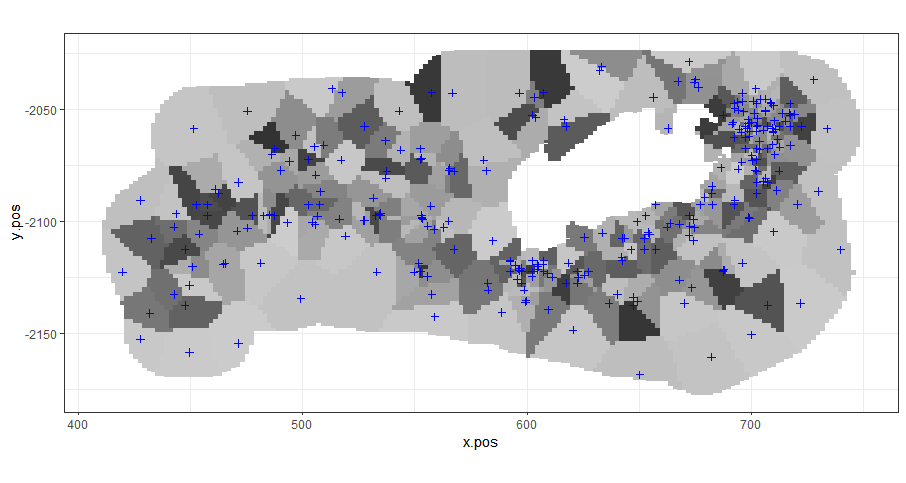
\includegraphics[width=0.9\linewidth]{suppimages/knotdatablocks}
\caption{Figure showing the knot locations (blue crosses) and the colour shows the nearest knot on the pseudo absence grid.}
\label{fig:blocks}
\end{figure}


\newpage

% \section{Cross-Validation}

% The cross-validation metric used for the point process models is a $k$-fold procedure, which generates spatially separated training and testing folds by considering circular buffers around each observation location.  This uses the {\tt buffering} function from the R package {\tt blockCV} (Valavi et al 2019).  The size of the blocks was estimated using an empirical variogram.  In this case, the range was estimated to be 1.5km$^2$. Both presence points and pseudo-absence points are assigned to a block and each block is left out in turn which is equivalent to leave-one out cross validation (using presence points only).

% % \begin{figure}[!h]
% % \centering
% % \caption{Figure showing an example of random fold assignment. Ten folds are chosen with a block size of 10km$^2$.}
% % \includegraphics[width=0.9\linewidth]{images/cvblocksfoldsexample}
% % \label{fig:cvblocks}
% % \end{figure}


% For each fold, $f$, the following procedure is followed:

% \begin{enumerate}
%     \item {Update the model by setting the weights on the data in fold $f$ to zero (equivalent to a thinned process where $p$ is known). This means that the intensity function can be evaluated at all locations but that these locations do not contribute to the likelihood function:

% \begin{equation*}
%     l_f(\beta;\textbf{X}) = \sum_{i=1}^{N}p_iw_i(y_i \textrm{log}(\lambda(\textbf{X}_i)) - \lambda (\textbf{X}_i))
% \end{equation*}

% where \(\lambda(\textbf{X}_i))\) is the intensity at location \(i\),  $\boldsymbol{X}_i$ represents both the coordinates and the environmental covariates at location $i$, $N$ is the total number of points (presence and pseudo-absence), $\textbf{w} = \{w_1, \cdots, w_N\}$ are quadrature weights.

% \begin{align*}
%     y_i = \begin{cases}
%       \frac{1}{w_i} & \text{if $i$ is a presence location}\\
%       0 & \text{if $i$ is a pseudo-absence location}
%     \end{cases} 
% \end{align*}
 
%  Here we model the expected number of carcasses per square kilometre and so the weights for the pseudo-absence points are specified as the area of the study region, 37,872 km$^2$ (ENP plus the 20 km buffer) divided by the number of pseudo-absences ($\sim 3.9$). The weights for presence points are set to some small value ($10^{-6}$).

% \begin{align*}
%     p_i = \begin{cases}
%       0 & \text{for presence/absence points in fold $f$}\\
%       1 & \text{otherwise}
%     \end{cases} 
% \end{align*}
    
%     }
%     \item Make predictions to the validation data (fold $f$),
%     \item Calculate the absolute residual for fold $f$ by comparing the sum of the observed presences and the sum of the estimated intensities.
%     $$cv_f = (|O_f-E_f|)^2$$
% \end{enumerate}

% \noindent Thus the CV score is calculated as the mean of all fold scores:

% $$CV = \frac{\sum_{f=1}^F cv_f}{F}$$

% where $F$ is the number of presence points (in this case $F=320$).


% \noindent To obtain a range of plausible values for the CV score, the scores ($cv_f$) are sampled with replacement (size $F$) and 95\% percentile intervals for the CV score were calculated using 1000 replicates.

\vspace{2cm}

% Questions/Thoughts:

% \begin{enumerate}
%     \item After a trial run, this seems more stable than the previously tried spatial blocking folds. Its also quicker.
%     \item The CI's overlap far less between models which allows some distinction.
%     \item The order of models using the CV scores is similar to that seen by AIC/BIC scores. Different "best models" would be chosen by each score. However, the differences in information criterion scores between the models is far greater. for example, the difference between first and second best models for AIC is 30 points. Some images of fits below.
%     \item Does it make sense to only use presence points as the focus of each fold, especially if the buffer is small?  What about the model fit in "absence" areas?
%     \item Does re-sampling the scores make sense for getting CI's?
% \end{enumerate}

\section{Pseudo-absence Selection}

\begin{itemize}
    \item Grid spacings trialled: 5, 4, 3, 2, 1.5, 1.25 and 1 km
    \item SALSA2D specification
    \begin{itemize}
        \item knot grid: all non-duplicated presence locations
        \item start knot number: 10, 20, 30, 40
        \item min knots and max knots equal to start knot number. 
        \item distance metric: Euclidean
        \item basis: Gaussian and exponential
    \end{itemize}
    \item Fit models for each specification of grid, start knots and basis
    \item Evaluate the log-likelihood
    \item Select the coarsest resolution after which, an increase in resolution makes little difference to the likelihood. 
\end{itemize}

Figure \ref{fig:resolutionconvergence} shows the log-likelihood scores for the different parameterisations. The vertical dashed line indicates the best grid resolution; 2km$^2$.

\begin{figure}[!htb]
\centering
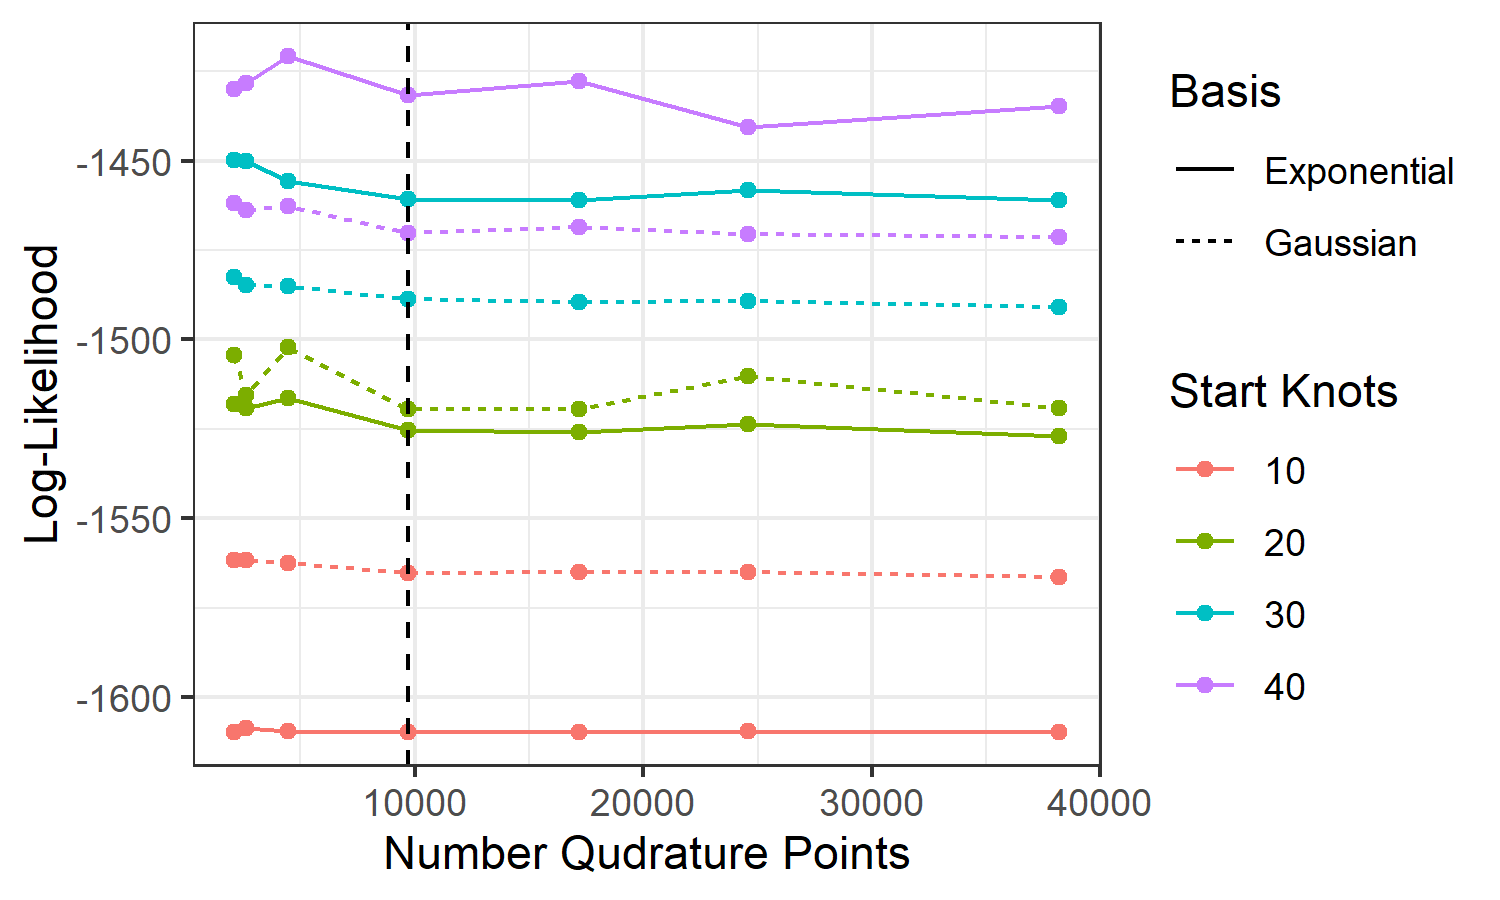
\includegraphics[width=0.9\linewidth]{suppimages/ppconverge.png}
\caption{Figure showing the convergence of the log-likelihood for for different spatial resolutions across multiple SALSA2D parameterisations.}
\label{fig:resolutionconvergence}
\end{figure}

\section{Estimated Intensities}

The following figures show the best models from the two different methodological frameworks and the four different parameterisations. The best models are selected using BIC for SALSA2D and AIC$_c$ weights for model averaging. Since, the two frameworks are compared using the log-likelihood, Figure \ref{fig:salsaloglik} shows the best log-likelihood selected models. 

% \begin{figure}[!hb]
% \centering
% \caption{Figure showing fitted intensity surfaces for the four SALSA2D models selected using BIC.}
% % \includegraphics[width=0.9\linewidth]{images/testoutputs}
% \label{fig:salsabic}
% \end{figure}

\begin{figure}[!htb]
\centering
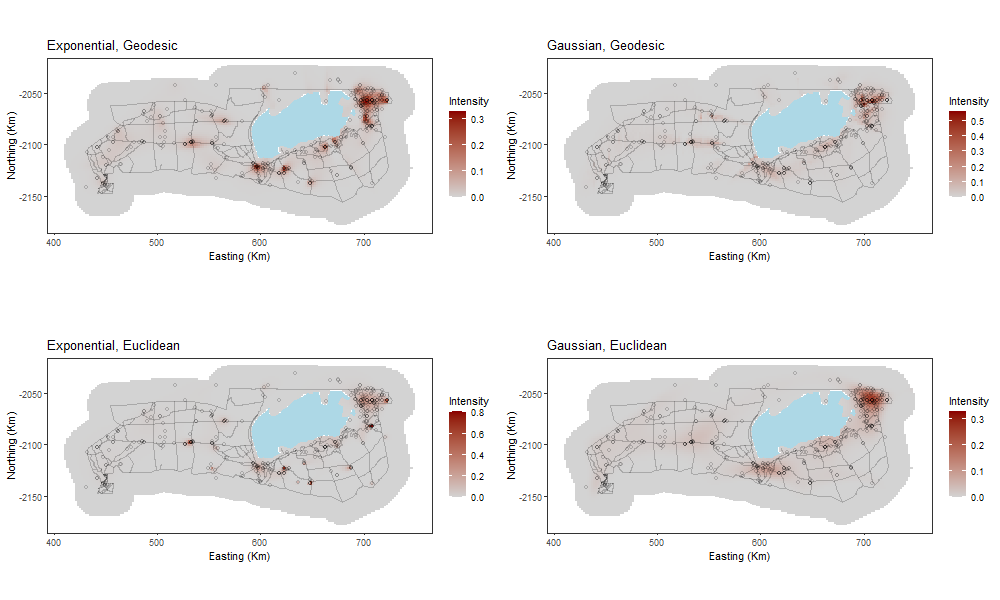
\includegraphics[width=0.9\linewidth]{suppimages/mrseapredplots_4methods.png}
\caption{Figure showing fitted intensity surfaces for the four SALSA2D models selected using log-likelihood.}
\label{fig:salsaloglik}
\end{figure}

\begin{figure}[!htb]
\centering
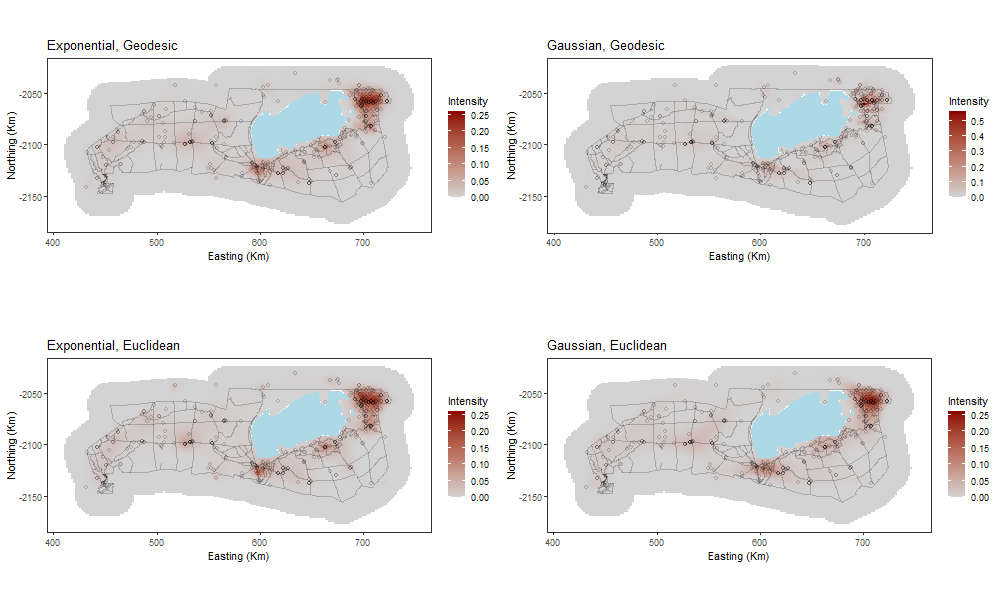
\includegraphics[width=0.9\linewidth]{suppimages/modelavgpredplots.png}
\caption{Figure showing the best model averaged outputs from the four different parametrisations and selected using AIC$_c$ model weights.}
\label{fig:modelavgall}
\end{figure}

\clearpage



\subsection*{SALSA2D outputs}

%\begin{table}[!htb]
\begin{table}[!htb]
\renewcommand{\arraystretch}{0.5}
\begin{tabular}{|l|l|r|r|r|r|r|}
\hline
Distance Type & Basis & \makecell[r]{Start \\Knots} & \makecell[l]{End \\Knots} & LogLik & BIC & \makecell[l]{Time \\(min)}\\
\hline
Euclidean & Exponential & 5 & 8 & -1528.5 & 3130.6 & 2.3\\
\hline
Euclidean & Exponential & 10 & 8 & -1509.1 & 3091.9 & 2.1\\
\hline
Euclidean & Exponential & 15 & 8 & -1517.0 & 3107.7 & 2.7\\
\hline
Euclidean & Exponential & 20 & 10 & -1504.6 & 3101.4 & 4.6\\
\hline
Euclidean & Exponential & 25 & 12 & -1486.3 & 3083.1 & 21.1\\
\hline
Euclidean & Exponential & 30 & 19 & -1445.0 & 3065.0 & 22.9\\
\hline
Euclidean & Exponential & 35 & 22 & -1438.7 & 3080.0 & 21.6\\
\hline
Euclidean & Exponential & 40 & 27 & -1407.7 & 3064.1 & 46.7\\
\hline
Euclidean & Exponential & 45 & 28 & -1376.8 & 3011.5 & 49.9\\
\hline
Euclidean & Exponential & 50 & 32 & -1374.5 & 3043.8 & 66.7\\
\hline
Euclidean & Exponential & 55 & 40 & -1318.0 & 3004.4 & 73.3\\
\hline
Euclidean & Exponential & 60 & 41 & -1301.6 & 2980.9 & 126.2\\
\hline
Euclidean & Gaussian & 5 & 7 & -1558.7 & 3181.9 & 1.4\\
\hline
Euclidean & Gaussian & 10 & 7 & -1572.4 & 3209.2 & 1.4\\
\hline
Euclidean & Gaussian & 15 & 8 & -1572.4 & 3218.4 & 2.1\\
\hline
Euclidean & Gaussian & 20 & 14 & -1533.1 & 3195.1 & 2.3\\
\hline
Euclidean & Gaussian & 25 & 15 & -1522.3 & 3182.8 & 18.4\\
\hline
Euclidean & Gaussian & 30 & 18 & -1515.9 & 3197.5 & 16.4\\
\hline
Euclidean & Gaussian & 35 & 28 & -1490.3 & 3238.6 & 37.6\\
\hline
Euclidean & Gaussian & 40 & 28 & -1489.0 & 3235.9 & 38.3\\
\hline
Euclidean & Gaussian & 45 & 34 & -1479.6 & 3272.5 & 31.6\\
\hline
Euclidean & Gaussian & 50 & 39 & -1471.3 & 3301.9 & 23.8\\
\hline
Euclidean & Gaussian & 55 & 47 & -1452.3 & 3337.4 & 38.1\\
\hline
Euclidean & Gaussian & 60 & 47 & -1451.6 & 3336.2 & 103.9\\
\hline
\end{tabular}
\caption{SALSA2D outputs for the Euclidean distance models\label{tab:outputseuc}}
\end{table}
%\end{table}

\begin{table}[!htb]
\begin{tabular}{|l|l|l|r|r|r|r|r|}
\hline
  & Distance Type & Basis & \makecell[r]{Start \\Knots} & \makecell[l]{End \\Knots} & LogLik & BIC & \makecell[l]{Time \\(min)}\\
\hline
25 & Geodesic & Exponential & 5 & 9 & -1502.5 & 3087.8 & 2.2\\
\hline
26 & Geodesic & Exponential & 10 & 5 & -1539.3 & 3124.7 & 2.7\\
\hline
27 & Geodesic & Exponential & 15 & 9 & -1492.5 & 3067.9 & 4.1\\
\hline
28 & Geodesic & Exponential & 20 & 12 & -1481.8 & 3074.1 & 5.1\\
\hline
29 & Geodesic & Exponential & 25 & 13 & -1472.7 & 3065.2 & 21.5\\
\hline
30 & Geodesic & Exponential & 30 & 15 & -1465.8 & 3069.8 & 18.6\\
\hline
31 & Geodesic & Exponential & 35 & 19 & -1448.3 & 3071.6 & 40.7\\
\hline
32 & Geodesic & Exponential & 40 & 25 & -1415.3 & 3060.9 & 13.5\\
\hline
33 & Geodesic & Exponential & 45 & 21 & -1427.4 & 3048.2 & 45.8\\
\hline
34 & Geodesic & Exponential & 50 & 32 & -1369.7 & 3034.2 & 62.7\\
\hline
35 & Geodesic & Exponential & 55 & 24 & -1398.1 & 3017.3 & 90.7\\
\hline
36 & Geodesic & Exponential & 60 & 28 & -1377.6 & 3013.1 & 103.7\\
\hline
37 & Geodesic & Gaussian & 5 & 8 & -1551.0 & 3175.6 & 1.2\\
\hline
38 & Geodesic & Gaussian & 10 & 6 & -1562.4 & 3180.1 & 0.9\\
\hline
39 & Geodesic & Gaussian & 15 & 7 & -1553.0 & 3170.6 & 0.8\\
\hline
40 & Geodesic & Gaussian & 20 & 11 & -1510.0 & 3121.4 & 18.5\\
\hline
41 & Geodesic & Gaussian & 25 & 14 & -1500.4 & 3129.8 & 19.8\\
\hline
42 & Geodesic & Gaussian & 30 & 15 & -1481.7 & 3101.6 & 13.9\\
\hline
43 & Geodesic & Gaussian & 35 & 21 & -1472.5 & 3138.4 & 33.7\\
\hline
44 & Geodesic & Gaussian & 40 & 25 & -1450.5 & 3131.3 & 8.7\\
\hline
45 & Geodesic & Gaussian & 45 & 26 & -1433.8 & 3107.0 & 46.9\\
\hline
46 & Geodesic & Gaussian & 50 & 31 & -1418.0 & 3121.7 & 40.9\\
\hline
47 & Geodesic & Gaussian & 55 & 32 & -1408.3 & 3111.3 & 76.8\\
\hline
48 & Geodesic & Gaussian & 60 & 33 & -1411.8 & 3127.5 & 26.6\\
\hline
\end{tabular}
\caption{SALSA2D outputs for the Geodesic models}
\label{tab:outputsgeo}
\end{table}

\begin{table}[!htb]
\begin{tabular}{|l|l|r|r|r|r|r|}
\hline
Distance Type & Basis & \makecell[r]{Start \\Knots} & \makecell[l]{End \\Knots} & LogLik & BIC & \makecell[l]{Time \\(min)}\\
\hline
Euclidean & Exponential & 60 & 41 & -1301.6 & 2980.9 & 126.2\\
\hline
Euclidean & Exponential & 55 & 40 & -1318.0 & 3004.4 & 73.3\\
\hline
Geodesic & Exponential & 50 & 32 & -1369.7 & 3034.2 & 62.7\\
\hline
Euclidean & Exponential & 50 & 32 & -1374.5 & 3043.8 & 66.7\\
\hline
Euclidean & Exponential & 45 & 28 & -1376.8 & 3011.5 & 49.9\\
\hline
Geodesic & Exponential & 60 & 28 & -1377.6 & 3013.1 & 103.7\\
\hline
Geodesic & Exponential & 55 & 24 & -1398.1 & 3017.3 & 90.7\\
\hline
Euclidean & Exponential & 40 & 27 & -1407.7 & 3064.1 & 46.7\\
\hline
Geodesic & Gaussian & 55 & 32 & -1408.3 & 3111.3 & 76.8\\
\hline
Geodesic & Gaussian & 60 & 33 & -1411.8 & 3127.5 & 26.6\\
\hline
\end{tabular}
\caption{Top 10 log-likelihood selected SALSA2D models}
\end{table}

\begin{table}[!htb]
    \centering
\begin{tabular}{|l|l|r|r|r|r|r|}
\hline
Distance Type & Basis & \makecell[r]{Start \\Knots} & \makecell[l]{End \\Knots} & LogLik & BIC & \makecell[l]{Time \\(min)}\\
\hline
Euclidean & Exponential & 60 & 41 & -1301.6 & 2980.9 & 126.2\\
\hline
Euclidean & Exponential & 55 & 40 & -1318.0 & 3004.4 & 73.3\\
\hline
Euclidean & Exponential & 45 & 28 & -1376.8 & 3011.5 & 49.9\\
\hline
Geodesic & Exponential & 60 & 28 & -1377.6 & 3013.1 & 103.7\\
\hline
Geodesic & Exponential & 55 & 24 & -1398.1 & 3017.3 & 90.7\\
\hline
Geodesic & Exponential & 50 & 32 & -1369.7 & 3034.2 & 62.7\\
\hline
Euclidean & Exponential & 50 & 32 & -1374.5 & 3043.8 & 66.7\\
\hline
Geodesic & Exponential & 45 & 21 & -1427.4 & 3048.2 & 45.8\\
\hline
Geodesic & Exponential & 40 & 25 & -1415.3 & 3060.9 & 13.5\\
\hline
Euclidean & Exponential & 40 & 27 & -1407.7 & 3064.1 & 46.7\\
\hline
\end{tabular}
\caption{Top 10 BIC selected SALSA2D models.}
    \label{tab:my_label}
\end{table}

\clearpage

\subsection*{Model Averaged Selected Models}

\begin{itemize}
    \item $k$ = number of knots
    \item $r$ = effective radius sequence number
    \item $w$ = AIC$_c$ model averaging weight
\end{itemize}

\begin{verbatim}
$expeuc
   k r w
1 50 1 1

$expgeo
    k  r           w
1  45  3 0.003343363
2  50  1 0.131329653
3  50  3 0.070500968
4  50  4 0.070848736
5  50  5 0.058365475
6  50  6 0.055646771
7  50  7 0.055112831
8  50  8 0.055009183
9  50  9 0.054987913
10 50 10 0.054925003
11 60  1 0.389930105

$gauseuc
   k r           w
1 55 2 0.006596805
2 55 3 0.052268277
3 55 4 0.062721223
4 55 5 0.025132387
5 60 2 0.107459248
6 60 3 0.566550328
7 60 4 0.159010615
8 60 5 0.020261116

$gausgeo
   k r          w
1 60 6 0.98712668
2 60 7 0.01287332
\end{verbatim}

% To obtain a range of plausible values for the CV score, the process is repeated with a new block structure (by allowing a horizontal and vertical adjustment) and new random assignment of blocks to folds. For this paper, the 95\% percentile intervals for the CV score were calculated using 100 replicates. 

% blocksize=10
% fulldata:
%      1    2    3    4    5    6    7    8    9   10
%   0  960  960  930  987 1013 1000  958  993  931 958
%   1   41   19   45   20   36   23   15   31   41  49

% leaving out fold 1:
%      1    2    3    4    5    6    7    8    9   10
%   0  960  960  930  987 1013 1000  958  993  931 958
%   1    0   19   45   20   36   23   15   31   41  49

% \begin{figure}[!h]
% \centering
% \caption{Figure showing an example of random fold assignment (coloured blocks). Ten folds are chosen with a block size of 10km$^2$. The coloured dots are the presence points. The black dots show the presence points removed in fold 1 (orange blocks)}
% \includegraphics[width=0.9\linewidth]{images/cvblocks_points}
% \label{fig:cvblockspopints}
% \end{figure}

\section{Full Analysis Covariate Information}

\subsection*{Rainfall calculation} 

Fit a high dimensional smooth term to 156 locations of annual rainfall from 1999 to 2015 (2016/17 unavailable at the time of modelling) to interpolate values for the presence locations and pseudo-absence grid.

\begin{verbatim}
require(mgcv)
fit<-gam(meanrain ~ s(x.pos, y.pos,fx = TRUE, k=150), data=rainfall2)
analysisdat$meanrain<-predict(object = fit, 
                    newdata = data.frame(x.pos = analysisdat$x.pos, 
                                        y.pos = analysisdat$y.pos))
\end{verbatim}

The results of the interpolation model are shown in Figure \ref{fig:covariates}

\begin{figure}[!htb]
\centering
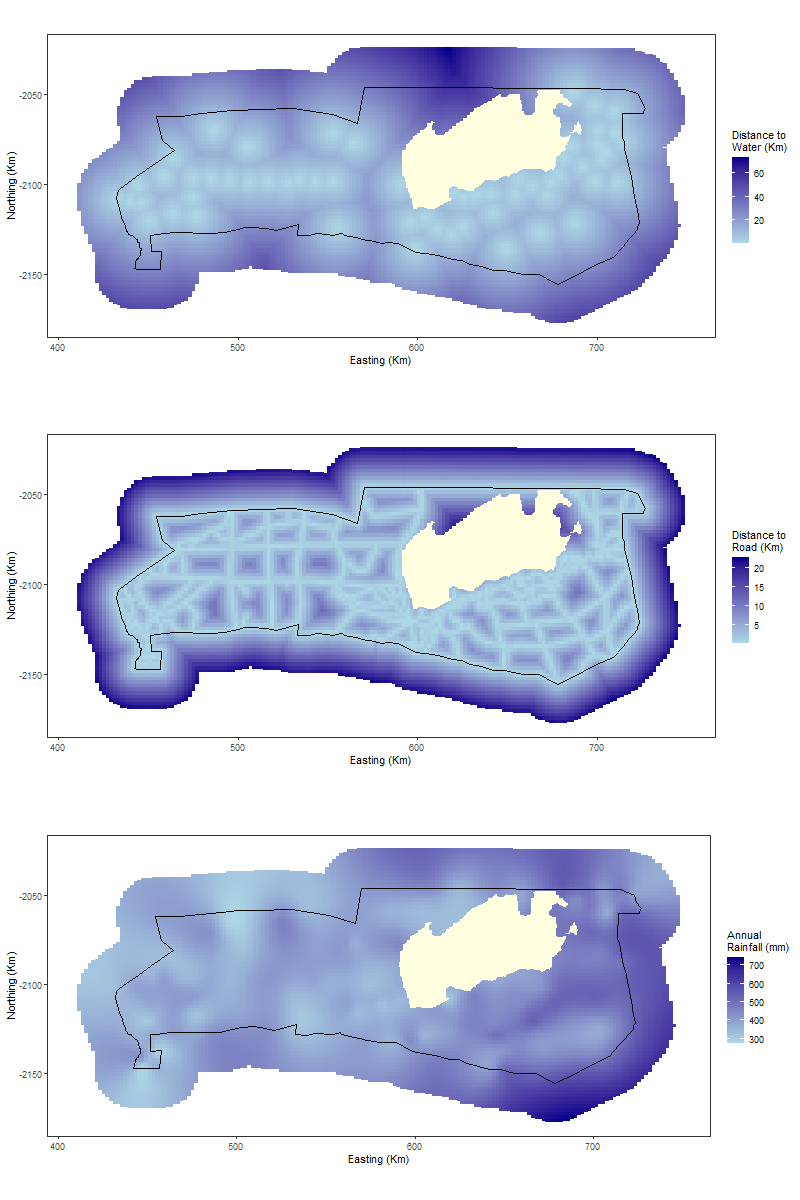
\includegraphics[width=0.9\linewidth]{suppimages/Mike_covardata.png}
\caption{Figure showing the covariate data in the study region. Distance to water (top), distance to roads (centre) and interpolated annual rainfall (bottom).}
\label{fig:covariates}
\end{figure}


\end{document}

